% ---
% Chapter 3
% ---
\chapter{A theory for CSP in Coq}
\label{chapter:csp_coq}
% ---

The \autoref{chapter:background} provided an overview of the essential concepts for understanding the implementation of the \CSPcoq{} language, setting the scene for an in-depth explanation of the language developed in this work. That being said, \autoref{chapter:csp_coq} will explain how each of these concepts combined together made it possible to develop a theory of communicating sequential processes in Coq proof assistant. The \autoref{section:syntax} discusses the implementation of the language's abstract and concrete syntax, whereas \autoref{section:sos} explains how the SOS style of defining language semantics translates into Coq as an inductive declaration. Furthermore, \autoref{section:lts} provides details on both functional and inductive definitions of LTS, along with further explanation on the GraphViz software integration. Finally, \autoref{section:traces} guides the reader through the definition of traces refinement as an executable property and also presents randomized testing based on this property using QuickChick plugin.

% ---
\section{Syntax}
\label{section:syntax}
% ---

The \CSPcoq{} language provides support to all process constructors and operations discussed in \autoref{section:csp}. Those include the processes $ \mathit{\STOP} $ and $ \mathit{\SKIP} $, and the operations event prefix, external choice, internal choice, alphabetized parallel, generalized parallel, interleave, sequential composition, and event hiding. This section introduces the reader to the implementation of both the abstract and concrete syntax of the \CSPcoq{} language in Coq.

% ---
\subsection{Abstract syntax}
% ---

In order to define all these CSP operations in Coq, we declared the following inductive types: \emph{event}, \emph{event\_tau\_tick}, \emph{channel}, \emph{alphabet}, \emph{proc\_body}, and \emph{proc\_def}. The type \emph{event} represents all external events. As we said before, external events are all events that are neither internal ($ \tau $) nor indicate termination ($ \tick $). On the other hand, the type \emph{event\_tau\_tick} provides not only a constructor for the external events, but also for the especial events $ \tau $ and $ \tick $.

For describing a set of external events, we have the \emph{channel} and \emph{alphabet} types. They are syntactically equivalent, the difference between these two constructors being purely semantic: the \emph{channel} type is used to account for all external events that may be communicated in a \CSPcoq{} specification, while the constructor provided by the \emph{alphabet} type is applied, for example, to enumerate all external events in a process interface in an alphabetized parallel combination.

The \emph{proc\_body} and \emph{proc\_def} types describe, respectively, the constructors for the operations we mentioned earlier in the beginning of this subsection, and the process attribution statement. The constructors available for the \emph{proc\_body} type allow us to combine processes in order to create more complex ones, while the \emph{proc\_def} type provides a constructor that makes it possible to identify a process by a string, and that is, to give it a name.

The last element from the CSP syntax that we described is the \emph{specification} type. A CSP specification can be perceived as a file containing multiple channels of events and process declarations. Ultimately, it is a context that holds information such as all the events that can be performed, and all process and corresponding definitions that compose a system. The way we introduce this concept in \CSPcoq{} is via a record type. Records are constructions that allow the definition of a set of attributes and propositions that must be satisfied in order to successfully define this structure.

To illustrate the abstract syntax defined via inductive types in Coq, consider the \CSPM{} processes
\
\begin{flushleft}
	PRINTER := accept -> print -> STOP

	PARKING\_PERMIT\_MCH := TICKET [ \{cash, ticket\} || \{cash, change\} ] CHANGE
\end{flushleft}
\
and their representations in \CSPcoq{} language

\begin{flushleft}
	Proc ``PRINTER'' (ProcPrefix (Event ``accept'') (ProcPrefix (Event ``print'') STOP))
\end{flushleft}

\begin{tabbing}
	\hspace*{1em}\= \hspace*{2em} \= \kill
	Proc ``PARKING\_PERMIT\_MCH'' (\\
	\>	ProcAlphaParallel (ProcRef ``TICKET'') (ProcRef ``CHANGE'')\\
	\>	(Alphabet (set\_add event\_dec ``cash'' (set\_add event\_dec ``ticket'' (empty\_set event))))\\
	\>	(Alphabet (set\_add event\_dec ``cash'' (set\_add event\_dec ``change'' (empty\_set event))))\\
	)
\end{tabbing}

As one might notice from the examples above, the abstract syntax -- though it dictates how well-formed expressions are constructed -- is not a pleasant way of writing statements or at least reading them. For that matter, we need a more convenient notation. One that resembles the \CSPM{} operators and, therefore, facilitates both implementation and understanding of \CSPcoq{} processes and specifications.

% ---
\subsection{Concrete syntax}
% ---

In order to define a more appropriate notation for the \CSPcoq{} language, the proof assistant's \coqdockw{Notation} command was used. This command allows the declaration of a new symbolic notation for an existing definition. The examples bellow demonstrate how this command is used to assign symbols (operators) to previously defined constructors.

\begin{coqdoccode}
	\coqdocnoindent
	\coqdockw{Notation} ``a \texttt{-{}-}> P'' := (\coqdocvar{ProcPrefix} \coqdocvar{a} \coqdocvar{P}) (\coqdoctac{at} \coqdockw{level} 80, \coqdoctac{right} \coqdockw{associativity}).\coqdoceol
	\coqdocnoindent
	\coqdockw{Notation} ``P [] Q'' := (\coqdocvar{ProcExtChoice} \coqdocvar{P} \coqdocvar{Q}) (\coqdoctac{at} \coqdockw{level} 90, \coqdoctac{left} \coqdockw{associativity}).\coqdoceol
	\coqdocnoindent
	\coqdockw{Notation} ``P [[ A \symbol{92}\symbol{92} B ]] Q'' := (\coqdocvar{ProcAlphaParallel} \coqdocvar{P} \coqdocvar{Q} (\coqdocvar{Alphabet} \coqdocvar{A}) (\coqdocvar{Alphabet} \coqdocvar{B})) (\coqdoctac{at} \coqdockw{level} 90, \coqdockw{no} \coqdockw{associativity}).\coqdoceol
\end{coqdoccode}

Along with the assignment of a notation symbol, we can specify its \emph{precedence level} and its \emph{associativity}. The precedence level helps Coq parse compound expressions, whereas the associativity setting helps to disambiguate expressions containing multiple occurrences of the same symbol. Coq uses precedence levels from 0 to 100, and left, right, or no associativity.

In the command lines above, the prefix operation has the higher precedence among all three operators and associates to the right. On the other hand, the external choice has a left associativity while the alphabetized parallel operator does not associates at all, meaning that brackets are necessary to create a compound expression with multiple parallel operations.

Then, we can use these symbols to rewrite the process examples from the previous subsection in a much more friendly and recognizable way:

\begin{flushleft}
	``PRINTER'' ::= ``accept'' \texttt{-{}-}> ``print'' \texttt{-{}-}> STOP

	``MACHINE'' ::= ProcRef ``TICKET'' [[ \{\{``cash'', ``ticket''\}\} \textbackslash\textbackslash \ \{\{``cash'', ``change''\}\} ]] ProcRef ``CHANGE''
\end{flushleft}

The \autoref{tab:cspm-csp_coq} displays a comparison between the \CSPM{} operators we discussed and the \CSPcoq{} language concrete syntax, achieved via Coq's \coqdockw{Notation} command:

\begin{table}[htb]
	\begin{center}
		\caption[The \CSPcoq{} concrete syntax]{The \CSPcoq{} concrete syntax.}
		\label{tab:cspm-csp_coq}
		\begin{tabular}{ |l|c|c| }
			\hline
			Constructor & \CSPM{} & \CSPcoq{} \\
			\hline
			Stop & STOP & STOP \\ [0.5ex]
			Skip & SKIP & SKIP \\ [0.5ex]
			Event prefix & e -> P & e \texttt{-{}-}> P \\  [0.5ex]
			External choice & P [] Q & P [] Q \\  [0.5ex]
			Internal choice & P |$ \sim $| Q & P |$ \sim $| Q \\ [0.5ex]
			Alphabetized parallel & P [A || B] Q & P [[A \textbackslash\textbackslash \ B]] Q \\ [0.5ex]
			Generalized parallel & P [| A |] Q & P [| A |] Q \\ [0.5ex]
			Interleave & P ||| Q & P ||| Q \\ [0.5ex]
			Sequential composition & P ; Q & P ;; Q \\ [0.5ex]
			Event hiding & P \textbackslash \ A & P \textbackslash \ A \\ [0.5ex]
			Process definition & P := Q & P ::= Q \\ [0.5ex]
			Process reference & P := e -> P & P ::= e \texttt{-{}-}> ProcRef ``P'' \\ [0.5ex]
			\hline
		\end{tabular}
	\end{center}
\end{table}

% ---
\section{Structured operational semantics}
\label{section:sos}
% ---

Now that we have a good understanding of not only how the abstract syntax but also a convenient notation of the \CSPcoq{} language were implemented in the proof assistant, it is time for us to discuss language semantics in Coq. All the declarations presented in this section are based on the inference rules discussed in \autoref{subsection:sos}. More specifically, we will address how those SOS rules from the previous chapter were ported into Coq's environment.

Recall the inductive definition of the evenness property exemplified in \autoref{section:coq}. In that example, it was possible to rewrite the inference rules for such property in terms of an inductive declaration in Coq, where each rule was translated into a propositional statement, more specifically, a logical implication. We will use the same approach to define the semantic rules of the \CSPcoq{} language.

Initially, a notation was defined to represent the SOS relation, in order to increase the readability of the inductive declaration. Thus, this new notation could be used in the constructors of the relational definition. The following Coq command line, similarly to the ones in the previous section, creates the infix notation ``S \# P // a ==> Q'', which can be pronounced ``in the specification \emph{S}, the process \emph{P}, after communicating \emph{a}, behaves like the process \emph{Q}'':

\begin{coqdoccode}
	\coqdocnoindent
	\coqdockw{Reserved Notation} ``S '\#' P '//' a '==>' Q'' (\coqdoctac{at} \coqdockw{level} 150, \coqdoctac{left} \coqdockw{associativity}).\coqdoceol
\end{coqdoccode}

To exemplify the usage of this notation inside the inductive definition, lets revisit the inference rule for the prefix operator:

\begin{prooftree}
	\AxiomC{}
	\UnaryInfC{$ (a \then P) \trans(2)[a] P $}
\end{prooftree}

This structure can be translated into Coq as a single constructor in the SOS relation:

\begin{coqdoccode}
	\coqdocnoindent
	\ensuremath{|} \coqdocvar{prefix\_rule} (\coqdocvar{S} : \coqdocvar{specification}) (\coqdocvar{P} : \coqdocvar{proc\_body}) (\coqdocvar{a} : \coqdocvar{event}) :\coqdoceol
	\coqdocindent{1.00em}
	\coqdocvar{S} \# (\coqdocvar{a} \texttt{-{}-}> \coqdocvar{P}) // \coqdocvar{Event} \coqdocvar{a} ==> \coqdocvar{P}\coqdoceol
\end{coqdoccode}

As far as the notation goes, this constructor can be interpreted as follows: given a specification $ S $, a process $ P $, and an event $ a $, in the context of $ S $, the process $ a \ \texttt{-{}-}> P $, after communicating event $ a $, behaves as the process $ P $. In other words, it is always true that, in the prefix operation $ a \then P $, after $ a $ is performed, the resulting process is $ P $.

Consider the following examples of constructors from the SOS relation. They refer to the external choice and alphabetized parallelism operations respectively. Note that each one of these operations need more than one inference rule in order to fully describe their semantics, as explained in \autoref{subsection:sos}. However, the definitions we are about to discuss only consider two of these rules: one that evaluates the external choice to the left side operand, and the joint step rule of the alphabetized parallelism operation, that represents the synchronization event between the processes.

\begin{coqdoccode}
	\coqdocnoindent
	\ensuremath{|} \coqdocvar{ext\_choice\_left\_rule} (\coqdocvar{S} : \coqdocvar{specification}) (\coqdocvar{P} \coqdocvar{Q} : \coqdocvar{proc\_body}) :\coqdoceol
	\coqdocindent{1.00em}
	\coqdockw{\ensuremath{\forall}} (\coqdocvar{P'} : \coqdocvar{proc\_body}) (\coqdocvar{a} : \coqdocvar{event\_tau\_tick}),\coqdoceol
	\coqdocindent{3.00em}
	\ensuremath{\lnot} \coqdocvar{eq} \coqdocvar{a} \coqdocvar{Tau} \ensuremath{\rightarrow}\coqdoceol
	\coqdocindent{3.00em}
	(\coqdocvar{S} \# \coqdocvar{P} // \coqdocvar{a} ==> \coqdocvar{P'}) \ensuremath{\rightarrow}\coqdoceol
	\coqdocindent{3.00em}
	(\coqdocvar{S} \# \coqdocvar{P} [] \coqdocvar{Q} // \coqdocvar{a} ==> \coqdocvar{P'})\coqdoceol
	\coqdocnoindent
	\ensuremath{|} \coqdocvar{alpha\_parall\_joint\_rule} (\coqdocvar{S} : \coqdocvar{specification}) (\coqdocvar{P} \coqdocvar{Q} : \coqdocvar{proc\_body}) (\coqdocvar{A} \coqdocvar{B} : \coqdoctac{set} \coqdocvar{event}) :\coqdoceol
	\coqdocindent{1.00em}
	\coqdockw{\ensuremath{\forall}} (\coqdocvar{P'} \coqdocvar{Q'} : \coqdocvar{proc\_body}) (\coqdocvar{a} : \coqdocvar{event}),\coqdoceol
	\coqdocindent{3.00em}
	\coqdocvar{set\_In} \coqdocvar{a} (\coqdocvar{set\_inter} \coqdocvar{event\_dec} \coqdocvar{A} \coqdocvar{B}) \ensuremath{\rightarrow}\coqdoceol
	\coqdocindent{3.00em}
	(\coqdocvar{S} \# \coqdocvar{P} // \coqdocvar{Event} \coqdocvar{a} ==> \coqdocvar{P'}) \ensuremath{\rightarrow}\coqdoceol
	\coqdocindent{3.00em}
	(\coqdocvar{S} \# \coqdocvar{Q} // \coqdocvar{Event} \coqdocvar{a} ==> \coqdocvar{Q'}) \ensuremath{\rightarrow}\coqdoceol
	\coqdocindent{3.00em}
	\coqdocvar{S} \# \coqdocvar{P} [[ \coqdocvar{A} \symbol{92}\symbol{92} \coqdocvar{B} ]] \coqdocvar{Q} // \coqdocvar{Event} \coqdocvar{a} ==> \coqdocvar{P'} [[ \coqdocvar{A} \symbol{92}\symbol{92} \coqdocvar{B} ]] \coqdocvar{Q'}\coqdoceol
\end{coqdoccode}

The \coqdocvar{ext\_choice\_left\_rule} constructor encodes the inference rule that solves the external choice operation for the left operand. As we saw earlier, this behavior is described in the SOS by the rule \
\
\begin{prooftree}
	\AxiomC{$ P \trans(2)[a] P' $}
	\RightLabel{\quad ($ a \neq \tau $)}
	\UnaryInfC{$ P \extchoice Q \trans(2)[a] P' $}
\end{prooftree}
\
which translates into the logical proposition

\begin{coqdoccode}
	\coqdocnoindent
	\ensuremath{\lnot} \coqdocvar{eq} \coqdocvar{a} \coqdocvar{Tau} \ensuremath{\rightarrow}
	(\coqdocvar{S} \# \coqdocvar{P} // \coqdocvar{a} ==> \coqdocvar{P'}) \ensuremath{\rightarrow}
	(\coqdocvar{S} \# \coqdocvar{P} [] \coqdocvar{Q} // \coqdocvar{a} ==> \coqdocvar{P'})\coqdoceol
\end{coqdoccode}

In this statement, we can see that the first term corresponds to the side condition of the inference rule, which guarantees that the event in question is not the internal event $ \tau $. The second term is the main premise of the rule, ensuring that it is possible for the event $ a $ to evolve the process $ P $ into $ P' $ in the specification $ S $. Together, the side condition and hypothesis establish the necessary conditions to resolve the external choice operation to the left hand operand.

Similarly, the inference rule that defines the synchronous communication of an event by two processes combined by the alphabetized parallelism operation, is described in Coq by the constructor \coqdocvar{alpha\_parall\_joint\_rule}. This rule, as we can see from its sequent notation below, has a side condition which guarantees that the event in question belongs to the intersection of the processes interfaces. Furthermore, it has two premises, which ensure this event is able to evolve both operands of the combination, that is, the processE  on the left and right side of the parallelism operator can communicate the event.

\begin{prooftree}
	\AxiomC{$ P \trans(2)[a] P' $}
	\AxiomC{$ Q \trans(2)[a] Q' $}
	\RightLabel{\quad ($ a \in A^{\tick} \cap B^{\tick} $)}
	\BinaryInfC{$ P \parallel[A][B] Q \trans(2)[a] P' \parallel[A][B] Q' $}
\end{prooftree}

The side condition and the premises are rewritten in the inductive definition as antecedents of a logical implication:

\begin{coqdoccode}
	\coqdocnoindent
	\coqdocvar{set\_In} \coqdocvar{a} (\coqdocvar{set\_inter} \coqdocvar{event\_dec} \coqdocvar{A} \coqdocvar{B}) \ensuremath{\rightarrow}\coqdoceol
	\coqdocindent{1.00em}
	(\coqdocvar{S} \# \coqdocvar{P} // \coqdocvar{Event} \coqdocvar{a} ==> \coqdocvar{P'}) \ensuremath{\rightarrow}\coqdoceol
	\coqdocindent{1.00em}
	(\coqdocvar{S} \# \coqdocvar{Q} // \coqdocvar{Event} \coqdocvar{a} ==> \coqdocvar{Q'}) \ensuremath{\rightarrow}\coqdoceol
	\coqdocindent{1.00em}
	\coqdocvar{S} \# \coqdocvar{P} [[ \coqdocvar{A} \symbol{92}\symbol{92} \coqdocvar{B} ]] \coqdocvar{Q} // \coqdocvar{Event} \coqdocvar{a} ==> \coqdocvar{P'} [[ \coqdocvar{A} \symbol{92}\symbol{92} \coqdocvar{B} ]] \coqdocvar{Q'}\coqdoceol
\end{coqdoccode}

Note that this constructor does not consider the $ \tick $ event as a possible synchronization event between the processes, even though it is included in the inference rule (side condition) we saw above. The reason for this is that we defined another constructor, \coqdocvar{alpha\_parall\_tick\_joint\_rule}, dedicated exclusively to this joint step allowed by the termination event.

The last example of constructor we want to highlight from the inductive definition of the SOS is the \emph{process reference} operation. This constructor defines the rules for unfolding a process definition inside the body of another process:

\begin{coqdoccode}
	\coqdocnoindent
	\ensuremath{|} \coqdocvar{reference\_rule} (\coqdocvar{S} : \coqdocvar{specification}) (\coqdocvar{P} : \coqdocvar{proc\_body}) (\coqdocvar{name} : \coqdocvar{string}) :\coqdoceol
	\coqdocindent{1.00em}
	\coqdockw{\ensuremath{\forall}} (\coqdocvar{Q} : \coqdocvar{proc\_body}),\coqdoceol
	\coqdocindent{3.00em}
	\coqdocvar{eq} \coqdocvar{P} (\coqdocvar{ProcRef} \coqdocvar{name}) \ensuremath{\rightarrow}\coqdoceol
	\coqdocindent{3.00em}
	\coqdocvar{eq} (\coqdocvar{get\_proc\_body} \coqdocvar{S} \coqdocvar{name}) (\coqdocvar{Some} \coqdocvar{Q}) \ensuremath{\rightarrow}\coqdoceol
	\coqdocindent{3.00em}
	\coqdocvar{S} \# \coqdocvar{P} // \coqdocvar{Tau} ==> \coqdocvar{Q}\coqdoceol
\end{coqdoccode}

As we can see, there are two premises for successfully unfolding a definition. First, the process that needs unfolding must be of the form \coqdocvar{ProcRef} \coqdocvar{name}, where \coqdocvar{ProcRef} is a constructor of the type \coqdocvar{proc\_body}, and \coqdocvar{name} is a string that identifies the process in a specification. Second, the process referenced by \coqdocvar{ProcRef} \coqdocvar{name} must be defined in the specification. To that end, the function \coqdocvar{get\_proc\_body} searches for this definition inside the specification, while the equality ensures this search results in ``$ Some \ Q $'', where $ Q $ is a process body. It is important to emphasize that such definition differs from the one implemented by the FDR tool. This approach will allow an ill-formed recursion such as $ P := P $ to be declared in \CSPcoq{}, introducing a $ \tau $ action to represent the effort of unfolding the definition and, therefore, increasing the process LTS size.

% ---
\section{Labelled transition systems}
\label{section:lts}
% ---

Now that we can define syntactically and semantically correct CSP processes in Coq through the definitions we declared so far, we will introduce yet another way of implementing processes, based on the idea of labelled transition systems. This section will cover how the LTS concept was embedded in the proof assistant via functional and inductive definitions, and how \CSPcoq{} provides support to the GraphViz software, which enables a graph visualization of CSP processes.

A labelled transition system consists of a non-empty set of states $ S $, with a designated initial state $ P_{0} $, a set of labels $ L $, and a ternary relation $ P \trans[x] Q $ meaning that the state $ P $ can perform an action labelled $ x $ and move to state $ Q $. In Coq, we defined a LTS in two different and complementary ways: a computable function and a relation.

To illustrate these definitions, consider the following \CSPcoq{} specification:

\begin{coqdoccode}
	\coqdocnoindent
	\coqdockw{Definition} \coqdocvar{SPEC} : \coqdocvar{specification}.\coqdoceol
	\coqdocnoindent
	\coqdockw{Proof}.\coqdoceol
	\coqdocindent{1.00em}
	\coqdocvar{solve\_spec\_ctx\_rules} (\coqdoceol
	\coqdocindent{2.00em}
	\coqdocvar{Build\_Spec}\coqdoceol
	\coqdocindent{2.00em}
	[ \coqdocvar{Channel} \{\{``a'', ``b'', ``c''\}\} ]\coqdoceol
	\coqdocindent{2.00em}
	[ ``P'' ::= (``a'' -{}-> ``b'' -{}-> \coqdocvar{STOP}) [] (``c'' -{}-> \coqdocvar{STOP}) ]\coqdoceol
	\coqdocindent{1.00em}
	).\coqdoceol
	\coqdocnoindent
	\coqdockw{Defined}.\coqdoceol
\end{coqdoccode}

Initially, the process ``P'' can perform either ``a'' or ``c''. If ``a'' gets communicated, the external choice resolves to the process ``b'' -{}-> STOP, which can then perform ``b'' and finish the execution. On the other hand, if the event ``c'' gets communicated instead, then the combination resolves to the process STOP and also terminates. Therefore, we can list three transitions for the process ``P'': from state (``a'' -{}-> ``b'' -{}-> STOP) [] (``c'' -{}-> STOP) to state ``b'' -{}-> STOP with event ``a'', from state (``a'' -{}-> ``b'' -{}-> STOP) [] (``c'' -{}-> STOP) to state STOP with event ``c'', and from state ``b'' -{}-> STOP to state STOP with event ``b''. To better describe these transitions, we will be using the 3-tuple notation ($ P $, $ a $, $ Q $), where $ P $ is the source state, $ a $ is the action (event), and $ Q $ is the target state.

We can apply the same intuition from this example in the implementation of a functional definition of LTS in Coq: starting with the initial state, compute all the immediate transitions available from this state, meaning all 3-tuples where the target states can be reached in one step from $ S_{0} $. Mark the initial state as ``visited'' and any other state discovered in the previous step as ``not visited''. Then, repeat this step for each unvisited state until there are no states to be visited anymore, keeping track of the states you have already visited and the ones that haven't been visited yet.

Let \coqdocvar{compute\_ltsR} be the function yielded by this algorithm, the following Coq command outputs the set of transitions from the LTS of the process ``P'':

\begin{coqdoccode}
	\coqdocnoindent
	\coqdockw{Compute} \coqdocvar{compute\_ltsR} \coqdocvar{SPEC} ``P'' 1000.\coqdoceol
\end{coqdoccode}

\begin{flushleft}
	Output:
\end{flushleft}

\begin{tabbing}
	\hspace*{2.5em}\= \hspace*{2em} \= \kill
	= Some\\
	\>	[(``a'' -{}-> ``b'' -{}-> STOP [] ``c'' -{}-> STOP, Event ``a'', ``b'' -{}-> STOP);\\
	\>	(``a'' -{}-> ``b'' -{}-> STOP [] ``c'' -{}-> STOP, Event ``c'', STOP);\\
	\>	(``b'' -{}-> STOP, Event ``b'', STOP)]\\
	: option (set transition)
\end{tabbing}

Note that we added an integer as the third parameter of the function \coqdocvar{compute\_ltsR}. Since every recursive definition (\coqdockw{Fixpoint}) in Coq must have an argument that explicitly decreases in each recursive call to ensure termination, the third parameter fulfills this premise. Therefore, the number of recursive calls is limited in order to prevent endless computations: this function only returns a set of transitions when it's able to visit all the states of the LTS before reaching the limit.

Once we have our result, we may still want to check whether this set of transitions is indeed the LTS of the process in question. One way to prove this is by demonstrating that for every process $ P $ and $ Q $, and event $ a $, $ P $ behaves like $ Q $ after communicating $ a $ if, and only if, the 3-tuple ($ P $, $ a $, $ Q $) belongs to the set of transitions. In other words, if $ T $ is the set of transitions in the LTS representation of the process $ P $, then every possible communication of $ P $ -- and its components (inner processes) -- is present in $ T $, and every transition in $ T $ is a valid communication of process $ P $ (or the sub-processes that make up $ P $). With that in mind, an inductive definition might be useful to prove this kind of assertion.

\begin{coqdoccode}
	\coqdocnoindent
	\coqdockw{Inductive} \coqdocvar{ltsR'} :\coqdoceol
	\coqdocindent{1.00em}
	\coqdocvar{specification} \ensuremath{\rightarrow} \coqdoceol
	\coqdocindent{1.00em}
	\coqdoctac{set} \coqdocvar{transition} \ensuremath{\rightarrow} \coqdoceol
	\coqdocindent{1.00em}
	\coqdoctac{set} \coqdocvar{proc\_body} \ensuremath{\rightarrow} \coqdoceol
	\coqdocindent{1.00em}
	\coqdoctac{set} \coqdocvar{proc\_body} \ensuremath{\rightarrow} \coqdoceol
	\coqdocindent{1.00em}
	\coqdockw{Prop} :=\coqdoceol
	\coqdocindent{1.00em}
	\ensuremath{|} \coqdocvar{lts\_empty\_rule} (\coqdocvar{S} : \coqdocvar{specification}) (\coqdocvar{visited} : \coqdoctac{set} \coqdocvar{proc\_body}) :\coqdoceol
	\coqdocindent{3.00em}
	\coqdocvar{ltsR'} \coqdocvar{S} \coqdocvar{nil} \coqdocvar{nil} \coqdocvar{visited}\coqdoceol
	\coqdocindent{1.00em}
	\ensuremath{|} \coqdocvar{lts\_inductive\_rule}\coqdoceol
	\coqdocindent{4.00em}
	(\coqdocvar{S} : \coqdocvar{specification})\coqdoceol
	\coqdocindent{4.00em}
	(\coqdocvar{T} : \coqdoctac{set} \coqdocvar{transition})\coqdoceol
	\coqdocindent{4.00em}
	(\coqdocvar{P} : \coqdocvar{proc\_body})\coqdoceol
	\coqdocindent{4.00em}
	(\coqdocvar{tl} \coqdocvar{visited} : \coqdoctac{set} \coqdocvar{proc\_body}) :\coqdoceol
	\coqdocindent{3.00em}
	\coqdockw{let} \coqdocvar{T'} := \coqdocvar{transitions\_from} \coqdocvar{P} \coqdocvar{T} \coqdoctac{in}\coqdoceol
	\coqdocindent{3.00em}
	\coqdockw{let} \coqdocvar{T'{}'} := \coqdocvar{set\_diff} \coqdocvar{transition\_eq\_dec} \coqdocvar{T} \coqdocvar{T'} \coqdoctac{in}\coqdoceol
	\coqdocindent{3.00em}
	\coqdockw{let} \coqdocvar{visited'} := \coqdocvar{set\_add} \coqdocvar{proc\_body\_eq\_dec} \coqdocvar{P} \coqdocvar{visited} \coqdoctac{in}\coqdoceol
	\coqdocindent{3.00em}
	\coqdockw{let} \coqdocvar{to\_visit} := \coqdocvar{set\_diff} \coqdocvar{proc\_body\_eq\_dec}\coqdoceol
	\coqdocindent{12.00em}
	(\coqdocvar{set\_union} \coqdocvar{proc\_body\_eq\_dec} \coqdocvar{tl} (\coqdocvar{target\_proc\_bodies} \coqdocvar{T'}))\coqdoceol
	\coqdocindent{12.00em}
	\coqdocvar{visited'} \coqdoctac{in}\coqdoceol
	\coqdocindent{3.00em}
	(\coqdockw{\ensuremath{\forall}} (\coqdocvar{a} : \coqdocvar{event\_tau\_tick}) (\coqdocvar{P'} : \coqdocvar{proc\_body}),\coqdoceol
	\coqdocindent{4.50em}
	(\coqdocvar{S} \# \coqdocvar{P} // \coqdocvar{a} ==> \coqdocvar{P'}) \ensuremath{\leftrightarrow} \coqdocvar{In} (\coqdocvar{P},\coqdocvar{a},\coqdocvar{P'}) \coqdocvar{T'}) \ensuremath{\rightarrow}\coqdoceol
	\coqdocindent{3.00em}
	\coqdocvar{ltsR'} \coqdocvar{S} \coqdocvar{T'{}'} \coqdocvar{to\_visit} \coqdocvar{visited'} \ensuremath{\rightarrow}\coqdoceol
	\coqdocindent{3.00em}
	\coqdocvar{ltsR'} \coqdocvar{S} \coqdocvar{T} (\coqdocvar{P} :: \coqdocvar{tl}) \coqdocvar{visited}.\coqdoceol
	\coqdocemptyline
	\coqdocnoindent
	\coqdockw{Definition} \coqdocvar{ltsR} (\coqdocvar{S} : \coqdocvar{specification}) (\coqdocvar{name} : \coqdocvar{string}) (\coqdocvar{T} : \coqdoctac{set} \coqdocvar{transition}) : \coqdockw{Prop} :=\coqdoceol
	\coqdocindent{1.00em}
	\coqdockw{match} \coqdocvar{get\_proc\_body} \coqdocvar{S} \coqdocvar{name} \coqdockw{with}\coqdoceol
	\coqdocindent{1.00em}
	\ensuremath{|} \coqdocvar{Some} \coqdocvar{body} \ensuremath{\Rightarrow} \coqdocvar{NoDup} \coqdocvar{T} \ensuremath{\land} \coqdocvar{ltsR'} \coqdocvar{S} \coqdocvar{T} [\coqdocvar{body}] \coqdocvar{nil}\coqdoceol
	\coqdocindent{1.00em}
	\ensuremath{|} \coqdocvar{None} \ensuremath{\Rightarrow} \coqdocvar{False}\coqdoceol
	\coqdocindent{1.00em}
	\coqdockw{end}.\coqdoceol
\end{coqdoccode}

The constructor \coqdocvar{lts\_empty\_rule} implies that the LTS relation holds when there are neither states to be visited nor transitions to validate anymore. On the other hand, the inductive step is described by the constructor \coqdocvar{lts\_inductive\_rule}, which proposes that $ T $ represents the set of transitions of the LTS of process $ P $ if the following two premises are satisfied:
\begin{itemize}
	\item Let $ T' $ be the subset of $ T $ containing all transitions from state $ P $, $ P \trans[a] Q \iff (P, a, Q) \in T'$;
	\item Let $ T'' $ be the set of all remaining transitions and $ S $ the set of states yet to be visited (union of the set of new states that can be reached from $ P $ and other unvisited states), the LTS relation must hold also for the sets $ T'' $ and $ S $.
\end{itemize}

% ---
\subsection{GraphViz integration}
% ---

GraphViz is an open source graph visualization software that takes descriptions of graphs in a simple text language -- in our case, the DOT language -- and make diagrams in useful formats, such as images, SVG, and PDF. Moreover, this tool allows the customization of these diagrams, such as options for colors, fonts, hyperlinks, and custom node shapes. Providing support for this software enables \CSPcoq{} programmers to generate a graph from the description of a LTS with one line of command. That way, the behavior of a process may be inspected and analyzed more easily, since a visual representation will be available.

In order to build the description of a graph in DOT language, it is necessary to define a mapping of the constructors of \coqdocvar{event\_tau\_tick} and \coqdocvar{proc\_body} types to the \coqdocvar{string} type. That way, it will be possible to convert each tuple from the LTS into a statement that corresponds to a transition of a graph in DOT syntax. One way to achieve this in Coq is through the \coqdockw{Coercion} command, which assigns a conversion function that maps an expression of one type into another.

Consider the following coercion from type \coqdocvar{event\_tau\_tick} to type \coqdocvar{string}:

\begin{coqdoccode}
	\coqdocnoindent
	\coqdockw{Definition} \coqdocvar{event\_tau\_tick\_to\_str} (\coqdocvar{e} : \coqdocvar{event\_tau\_tick}) : \coqdocvar{string} :=\coqdoceol
	\coqdocindent{1.00em}
	\coqdockw{match} \coqdocvar{e} \coqdockw{with}\coqdoceol
	\coqdocindent{1.00em}
	\ensuremath{|} \coqdocvar{Tau} \ensuremath{\Rightarrow} ``$ \tau $''\coqdoceol
	\coqdocindent{1.00em}
	\ensuremath{|} \coqdocvar{Tick} \ensuremath{\Rightarrow} ``$ \tick $''\coqdoceol
	\coqdocindent{1.00em}
	\ensuremath{|} \coqdocvar{Event} \coqdocvar{a} \ensuremath{\Rightarrow} \coqdocvar{a}\coqdoceol
	\coqdocindent{1.00em}
	\coqdockw{end}.\coqdoceol
	\coqdocemptyline
	\coqdocnoindent
	\coqdockw{Coercion} \coqdocvar{event\_tau\_tick\_to\_str} : \coqdocvar{event\_tau\_tick} >-> \coqdocvar{string}.\coqdoceol
\end{coqdoccode}

As we can see from the code snippet above, initially, we defined a function that takes an element of type \coqdocvar{event\_tau\_tick} and returns a string representation of that element. Then, a coercion between the two types is established: from this point on, Coq will convert an element of type \coqdocvar{event\_tau\_tick} into a string whenever it is necessary.

Once the coercions are configured, we can define a function to create the description of a graph in the DOT language from the set of tuples that make up the LTS. The intuition behind this function is as follows: the first tuple to be processed has its starting state identified as the graph's initial node (bold and red border), and each tuple -- the first included -- is rewritten as a DOT syntax transition statement. In other words, the tuple (P, e, Q) generates the string ``<P> -> <Q> [label = <e>];'', as shown in the definitions below:

\begin{coqdoccode}
	\coqdocnoindent
	\coqdockw{Fixpoint} \coqdocvar{generate\_dot'} (\coqdocvar{lts} : \coqdoctac{set} \coqdocvar{transition}) : \coqdocvar{string} :=\coqdoceol
	\coqdocindent{1.00em}
	\coqdockw{match} \coqdocvar{lts} \coqdockw{with}\coqdoceol
	\coqdocindent{1.00em}
	\ensuremath{|} \coqdocvar{nil} \ensuremath{\Rightarrow} ``''\coqdoceol
	\coqdocindent{1.00em}
	\ensuremath{|} (\coqdocvar{P}, \coqdocvar{e}, \coqdocvar{Q}) :: \coqdocvar{tl} \ensuremath{\Rightarrow} `` <'' ++ \coqdocvar{P} ++ ``> -> <'' ++ \coqdocvar{Q} ++ ``>'' ++ `` [label=<'' ++ \coqdocvar{e} ++ ``>];'' ++ (\coqdocvar{generate\_dot'} \coqdocvar{tl})\coqdoceol
	\coqdocindent{1.00em}
	\coqdockw{end}.\coqdoceol
	\coqdocemptyline
	\coqdocnoindent
	\coqdockw{Definition} \coqdocvar{style\_initial\_state} (\coqdocvar{P} : \coqdocvar{proc\_body}) : \coqdocvar{string} := ``<'' ++ \coqdocvar{P} ++ ``> [style=bold, color=red];''.\coqdoceol
	\coqdocemptyline
	\coqdocnoindent
	\coqdockw{Definition} \coqdocvar{generate\_dot} (\coqdocvar{lts} : \coqdocvar{option} (\coqdoctac{set} \coqdocvar{transition})) : \coqdocvar{string} :=\coqdoceol
	\coqdocindent{1.00em}
	\coqdockw{match} \coqdocvar{lts} \coqdockw{with}\coqdoceol
	\coqdocindent{1.00em}
	\ensuremath{|} \coqdocvar{Some} ((\coqdocvar{P}, \coqdocvar{e}, \coqdocvar{Q}) :: \coqdocvar{tl}) \ensuremath{\Rightarrow}\coqdoceol
	\coqdocindent{2.00em}
	``digraph LTS \{ '' ++ (\coqdocvar{style\_initial\_state} \coqdocvar{P}) ++ (\coqdocvar{generate\_dot'} ((\coqdocvar{P}, \coqdocvar{e}, \coqdocvar{Q}) :: \coqdocvar{tl})) ++ `` \}''\coqdoceol
	\coqdocindent{1.00em}
	\ensuremath{|} \coqdocvar{\_} \ensuremath{\Rightarrow} ``''\coqdoceol
	\coqdocindent{1.00em}
	\coqdockw{end}.\coqdoceol
\end{coqdoccode}

To demonstrate what these definitions can achieve, recall the process MACHINE from the section 3.1.2. Here is a complete definition of that process in \CSPcoq{}:

\begin{coqdoccode}
	\coqdocnoindent
	\coqdockw{Definition} \coqdocvar{PARKING\_PERMIT\_MCH} : \coqdocvar{specification}.\coqdoceol
	\coqdocnoindent
	\coqdockw{Proof}.\coqdoceol
	\coqdocindent{1.00em}
	\coqdocvar{solve\_spec\_ctx\_rules} (\coqdoceol
	\coqdocindent{2.00em}
	\coqdocvar{Build\_Spec}\coqdoceol
	\coqdocindent{2.00em}
	[ \coqdocvar{Channel} \{\{``cash'', ``ticket'', ``change''\}\} ]\coqdoceol
	\coqdocindent{2.00em}
	[ ``TICKET'' ::= ``cash'' -{}-> ``ticket'' -{}-> \coqdocvar{ProcRef} ``TICKET''\coqdoceol
	\coqdocindent{2.00em}
	; ``CHANGE'' ::= ``cash'' -{}-> ``change'' -{}-> \coqdocvar{ProcRef} ``CHANGE''\coqdoceol
	\coqdocindent{2.00em}
	; ``MACHINE'' ::= \coqdocvar{ProcRef} ``TICKET'' [[ \{\{``cash'', ``ticket''\}\} \symbol{92}\symbol{92} \{\{``cash'', ``change''\}\} ]] \coqdocvar{ProcRef} ``CHANGE'' ]\coqdoceol
	\coqdocindent{1.00em}
	).\coqdoceol
	\coqdocnoindent
	\coqdockw{Defined}.\coqdoceol
\end{coqdoccode}

To generate the description of the graph in DOT syntax for the process MACHINE, simply run this command in Coq:

\begin{coqdoccode}
	\coqdocnoindent
	\coqdockw{Compute} \coqdocvar{generate\_dot} (\coqdocvar{compute\_ltsR} \coqdocvar{PARKING\_PERMIT\_MCH} ``MACHINE'' 1000).\coqdoceol
\end{coqdoccode}

We can then save the string output to a file named LTS.gv and run the following command in a terminal with the GraphViz software installed:

\emph{\$ dot -Nlabel=``'' -Nshape=circle -Tjpeg LTS.gv -o LTS.jpeg}

The \autoref{image:machine_lts} shows the expected output: an image in JPEG format containing a graph -- with nodes shaped as circles and no labels -- that represents the process LTS:

\begin{figure}[htb]
	\caption[Example LTS: The process MACHINE]{Example LTS: The process MACHINE.}
	\label{image:machine_lts}
	\begin{center}
		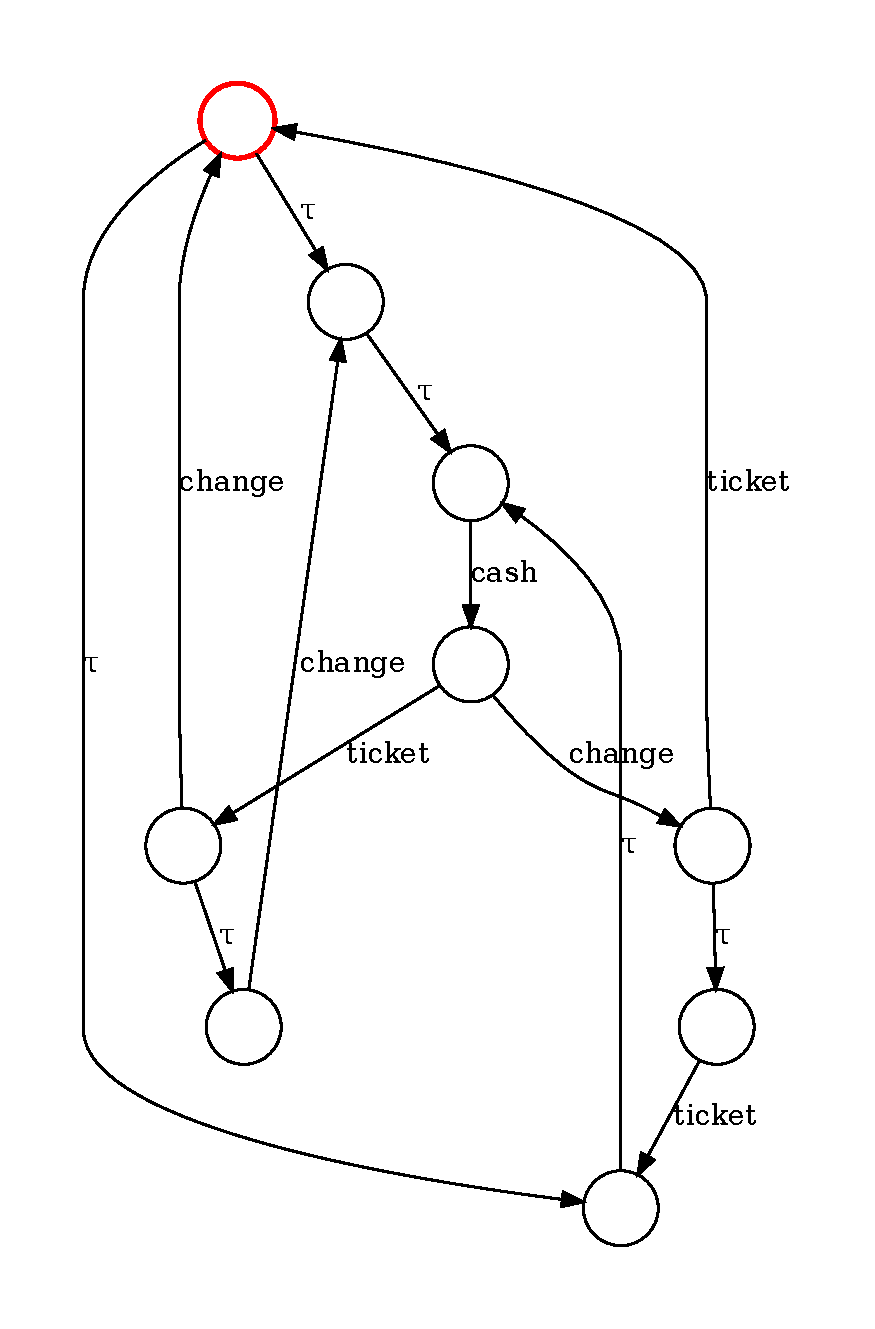
\includegraphics[scale=0.75]{images/parking_permit_mch_lts.pdf}
	\end{center}
\end{figure}

% ---
\section{Traces refinement}
\label{section:traces}
% ---

As we saw earlier in \autoref{subsection:traces-refinement}, a simple but effective way to analyze the behavior of a process is through the sequence of externally visible events such process is capable of performing over time. This communication history is called \emph{trace}. Using the concepts we saw previously, we may perceive trace as a list of actions that takes from one state to another in a LTS, or even the sequence of external events that one process can be communicate according to the operational semantics.

% ---
\subsection{Traces-related concepts}
% ---

Like the other types of CSP language we have discussed so far in this work, the trace also has its counterpart in \CSPcoq{}. It is defined in terms of a list of events that can be observed by the environment, that is, neither $ \tau $ nor $ \tick $ can be present in that list. This restriction is guaranteed in Coq by choosing the inductive type \coqdocvar{event} in the trace definition, instead of the type \coqdocvar{event\_tau\_tick}, which also includes internal and termination events. Below, we can check the definition in the proof assistant:

\begin{coqdoccode}
	\coqdocnoindent
	\coqdockw{Definition} \coqdocvar{trace} := \coqdocvar{list} \coqdocvar{event}.\coqdoceol
\end{coqdoccode}

After defining this type, we can then declare trace as a relationship between a process P and a list of events L, so that it is possible to make logical propositions that involve whether or not L is a trace of P. Initially, we can describe four rules of inference that govern this relationship:

% inserir regras de inferência na notação de barra
\begin{itemize}
	\item the empty list is a trace of any process;
	\begin{prooftree}
		\AxiomC{}
		\UnaryInfC{$ \mathit{trace} \ P \ nil $}
	\end{prooftree}
	\item a non-empty list L is a trace of a process P if the first element of L can be performed by P and the remaining events of this list is a trace of the process resulting from this communication;
	\begin{prooftree}
		\AxiomC{$ P \trans[h] Q $}
		\AxiomC{$ \mathit{trace} \ Q \ tl $}
		\RightLabel{\quad ($ h \notin \{\tick, \ \tau\} $)}
		\BinaryInfC{$ \mathit{trace} \ P \ (h :: tl) $}
	\end{prooftree}
	\item a list L is a trace of a process P if $ \tick $ can be performed by P and L is a trace of the process resulting from this communication;
	\begin{prooftree}
		\AxiomC{$ P \trans[\tick] Q $}
		\AxiomC{$ \mathit{trace} \ Q \ L $}
		\BinaryInfC{$ \mathit{trace} \ P \ L $}
	\end{prooftree}
	\item a list L is a trace of a process P if $ \tau $ can be performed by P and L is a trace of the process resulting from this communication.
	\begin{prooftree}
		\AxiomC{$ P \trans[\tau] Q $}
		\AxiomC{$ \mathit{trace} \ Q \ L $}
		\BinaryInfC{$ \mathit{trace} \ P \ L $}
	\end{prooftree}
\end{itemize}

Now, our knowledge of inductive declaration in Coq will be useful once again to embed these rules in the tool -- each one of these can be translated into a constructor from the \coqdocvar{traceR'} definition:

\begin{coqdoccode}
	\coqdocnoindent
	\coqdockw{Inductive} \coqdocvar{traceR'} : \coqdocvar{specification} \ensuremath{\rightarrow} \coqdocvar{proc\_body} \ensuremath{\rightarrow} \coqdocvar{trace} \ensuremath{\rightarrow} \coqdockw{Prop} :=\coqdoceol
	\coqdocindent{1.00em}
	\ensuremath{|} \coqdocvar{empty\_trace\_rule} (\coqdocvar{S} : \coqdocvar{specification}) (\coqdocvar{P} : \coqdocvar{proc\_body}) :\coqdoceol
	\coqdocindent{2.00em}
	\coqdocvar{traceR'} \coqdocvar{S} \coqdocvar{P} \coqdocvar{nil}\coqdoceol
	\coqdocindent{1.00em}
	\ensuremath{|} \coqdocvar{event\_trace\_rule} (\coqdocvar{S} : \coqdocvar{specification}) (\coqdocvar{P} \coqdocvar{P'} : \coqdocvar{proc\_body}) (\coqdocvar{h} : \coqdocvar{event}) (\coqdocvar{tl} : \coqdocvar{trace}) :\coqdoceol
	\coqdocindent{2.00em}
	(\coqdocvar{S} \# \coqdocvar{P} // \coqdocvar{Event} \coqdocvar{h} ==> \coqdocvar{P'}) \ensuremath{\rightarrow}\coqdoceol
	\coqdocindent{2.00em}
	\coqdocvar{traceR'} \coqdocvar{S} \coqdocvar{P'} \coqdocvar{tl} \ensuremath{\rightarrow}\coqdoceol
	\coqdocindent{2.00em}
	\coqdocvar{traceR'} \coqdocvar{S} \coqdocvar{P} (\coqdocvar{h}::\coqdocvar{tl})\coqdoceol
	\coqdocindent{1.00em}
	\ensuremath{|} \coqdocvar{tick\_trace\_rule} (\coqdocvar{S} : \coqdocvar{specification}) (\coqdocvar{P} \coqdocvar{P'} : \coqdocvar{proc\_body}) (\coqdocvar{t} : \coqdocvar{trace}) :\coqdoceol
	\coqdocindent{2.00em}
	(\coqdocvar{S} \# \coqdocvar{P} // \coqdocvar{Tick} ==> \coqdocvar{P'}) \ensuremath{\rightarrow}\coqdoceol
	\coqdocindent{2.00em}
	\coqdocvar{traceR'} \coqdocvar{S} \coqdocvar{P'} \coqdocvar{t} \ensuremath{\rightarrow}\coqdoceol
	\coqdocindent{2.00em}
	\coqdocvar{traceR'} \coqdocvar{S} \coqdocvar{P} \coqdocvar{t}\coqdoceol
	\coqdocindent{1.00em}
	\ensuremath{|} \coqdocvar{tau\_trace\_rule} (\coqdocvar{S} : \coqdocvar{specification}) (\coqdocvar{P} \coqdocvar{P'} : \coqdocvar{proc\_body}) (\coqdocvar{t} : \coqdocvar{trace}) :\coqdoceol
	\coqdocindent{2.00em}
	(\coqdocvar{S} \# \coqdocvar{P} // \coqdocvar{Tau} ==> \coqdocvar{P'}) \ensuremath{\rightarrow}\coqdoceol
	\coqdocindent{2.00em}
	\coqdocvar{traceR'} \coqdocvar{S} \coqdocvar{P'} \coqdocvar{t} \ensuremath{\rightarrow}\coqdoceol
	\coqdocindent{2.00em}
	\coqdocvar{traceR'} \coqdocvar{S} \coqdocvar{P} \coqdocvar{t}.\coqdoceol
	\coqdocemptyline
	\coqdocnoindent
	\coqdockw{Definition} \coqdocvar{traceR} (\coqdocvar{S} : \coqdocvar{specification}) (\coqdocvar{proc\_name} : \coqdocvar{string}) (\coqdocvar{t} : \coqdocvar{trace}) :=\coqdoceol
	\coqdocindent{1.00em}
	\coqdockw{match} (\coqdocvar{get\_proc\_body} \coqdocvar{S} \coqdocvar{proc\_name}) \coqdockw{with}\coqdoceol
	\coqdocindent{1.00em}
	\ensuremath{|} \coqdocvar{Some} \coqdocvar{body} \ensuremath{\Rightarrow} \coqdocvar{traceR'} \coqdocvar{S} \coqdocvar{body} \coqdocvar{t}\coqdoceol
	\coqdocindent{1.00em}
	\ensuremath{|} \coqdocvar{None} \ensuremath{\Rightarrow} \coqdocvar{False}\coqdoceol
	\coqdocindent{1.00em}
	\coqdockw{end}.\coqdoceol
\end{coqdoccode}

One might notice that the inference rules described above, in the order they were presented, correspond, respectively, to the constructors \coqdocvar{empty\_trace\_rule,} \coqdocvar{event\_trace\_rule}, \coqdocvar{tick\_trace\_rule}, and \coqdocvar{tau\_trace\_rule} of the \coqdocvar{traceR'} inductive definition.

This definition of trace as a relation, as well as the definition of operational semantics in the SOS style, allows us not only to make assertions like \emph{traceR S ``P'' L}, given a specification $ S $, a process $ P $ and a list of events $ L $, but also prove them in Coq by applying the constructors from the inductive declarations available.

It turns out that, not only these proofs, that verify the trace relationship between a process and a list of events, grow in proportion to the size of the list you want to check, they also become quite repetitive. Fortunately, this repetition allows us to define an algorithm to automatically prove assertions of this kind, and thus create a tactic macro for that purpose.

This algorithm can be defined as follows: if the goal is to prove the trace relation for an empty list, apply the rule \coqdocvar{empty\_trace\_rule} and fishing the proof, otherwise, try to make progress by applying each of the other three constructors of the \coqdocvar{traceR'} definition, making a recursive call afterwards. For goals which are operations described by the \CSPcoq{} semantics, try to make progress using the constructors applicable for that operation based on pattern matching, making once again a recursive call at the end of this step.

The following definition uses the Ltac language to describe this algorithm as a tactic macro that automatically proves statements of the kind \emph{traceR S ``P'' L}:

\begin{coqdoccode}
	\coqdocnoindent
	\coqdockw{Ltac} \coqdocvar{solve\_trace'} :=\coqdoceol
	\coqdocindent{1.00em}
	\coqdocvar{multimatch} \coqdockw{goal} \coqdockw{with}\coqdoceol
	\coqdocindent{1.00em}
	\ensuremath{|} \ensuremath{\vdash} \coqdocvar{traceR'} \coqdocvar{\_} \coqdocvar{\_} \coqdocvar{nil} \ensuremath{\Rightarrow} \coqdoctac{apply} \coqdocvar{empty\_trace\_rule}\coqdoceol
	\coqdocindent{1.00em}
	\ensuremath{|} \ensuremath{\vdash} \coqdocvar{traceR'} \coqdocvar{\_} \coqdocvar{\_} \coqdocvar{\_} \ensuremath{\Rightarrow}\coqdoceol
	\coqdocindent{2.00em}
	(\coqdoctac{eapply} \coqdocvar{tau\_trace\_rule}\coqdoceol
	\coqdocindent{2.00em}
	+ \coqdoctac{eapply} \coqdocvar{tick\_trace\_rule}\coqdoceol
	\coqdocindent{2.00em}
	+ \coqdoctac{eapply} \coqdocvar{event\_trace\_rule}); \coqdocvar{solve\_trace'}\coqdoceol
	\coqdocindent{1.00em}
	\ensuremath{|} \ensuremath{\vdash} \coqdocvar{\_} \# \coqdocvar{\_} --> \coqdocvar{\_} // \coqdocvar{\_} ==> \coqdocvar{\_} \ensuremath{\Rightarrow} \coqdoctac{apply} \coqdocvar{prefix\_rule}\coqdoceol
	\coqdocindent{1.00em}
	\ensuremath{|} \ensuremath{\vdash} \coqdocvar{\_} \# \coqdocvar{ProcRef} \coqdocvar{\_} // \coqdocvar{\_} ==> \coqdocvar{\_} \ensuremath{\Rightarrow} \coqdoctac{eapply} \coqdocvar{reference\_rule}; \coqdocvar{solve\_trace'}\coqdoceol
	\coqdocindent{1.00em}
	\ensuremath{|} \ensuremath{\vdash} \coqdocvar{\_} \# \coqdocvar{\_} [] \coqdocvar{\_} // \coqdocvar{\_} ==> \coqdocvar{\_} \ensuremath{\Rightarrow}\coqdoceol
	\coqdocindent{2.00em}
	(\coqdoctac{eapply} \coqdocvar{ext\_choice\_tau\_left\_rule}\coqdoceol
	\coqdocindent{2.00em}
	+ \coqdoctac{eapply} \coqdocvar{ext\_choice\_tau\_right\_rule}\coqdoceol
	\coqdocindent{2.00em}
	+ \coqdoctac{eapply} \coqdocvar{ext\_choice\_left\_rule}\coqdoceol
	\coqdocindent{2.00em}
	+ \coqdoctac{eapply} \coqdocvar{ext\_choice\_right\_rule}); \coqdocvar{solve\_trace'}\coqdoceol
	\coqdocindent{1.00em}
	\ensuremath{|} \ensuremath{\vdash} \coqdocvar{\_} \# \coqdocvar{\_} |\~{}| \coqdocvar{\_} // \coqdocvar{\_} ==> \coqdocvar{\_} \ensuremath{\Rightarrow}\coqdoceol
	\coqdocindent{2.00em}
	(\coqdoctac{eapply} \coqdocvar{int\_choice\_left\_rule}\coqdoceol
	\coqdocindent{2.00em}
	+ \coqdoctac{eapply} \coqdocvar{int\_choice\_right\_rule}); \coqdocvar{solve\_trace'}\coqdoceol
	\coqdocindent{1.00em}
	\ensuremath{|} \ensuremath{\vdash} \coqdocvar{\_} \# \coqdocvar{\_} [[ \coqdocvar{\_} \symbol{92}\symbol{92} \coqdocvar{\_} ]] \coqdocvar{\_} // \coqdocvar{\_} ==> \coqdocvar{\_} \ensuremath{\Rightarrow}\coqdoceol
	\coqdocindent{2.00em}
	(\coqdoctac{eapply} \coqdocvar{alpha\_parall\_tau\_indep\_left\_rule}\coqdoceol
	\coqdocindent{2.00em}
	+ \coqdoctac{eapply} \coqdocvar{alpha\_parall\_tau\_indep\_right\_rule}\coqdoceol
	\coqdocindent{2.00em}
	+ \coqdoctac{eapply} \coqdocvar{alpha\_parall\_tick\_joint\_rule}\coqdoceol
	\coqdocindent{2.00em}
	+ \coqdoctac{eapply} \coqdocvar{alpha\_parall\_joint\_rule}\coqdoceol
	\coqdocindent{2.00em}
	+ \coqdoctac{eapply} \coqdocvar{alpha\_parall\_indep\_left\_rule}\coqdoceol
	\coqdocindent{2.00em}
	+ \coqdoctac{eapply} \coqdocvar{alpha\_parall\_indep\_right\_rule}); \coqdocvar{solve\_trace'}\coqdoceol
	\coqdocindent{1.00em}
	\ensuremath{|} \ensuremath{\vdash} \coqdocvar{\_} \# \coqdocvar{\_} [| \coqdocvar{\_} |] \coqdocvar{\_} // \coqdocvar{\_} ==> \coqdocvar{\_} \ensuremath{\Rightarrow}\coqdoceol
	\coqdocindent{2.00em}
	(\coqdoctac{eapply} \coqdocvar{gener\_parall\_tau\_indep\_left\_rule}\coqdoceol
	\coqdocindent{2.00em}
	+ \coqdoctac{eapply} \coqdocvar{gener\_parall\_tau\_indep\_right\_rule}\coqdoceol
	\coqdocindent{2.00em}
	+ \coqdoctac{eapply} \coqdocvar{gener\_parall\_tick\_joint\_rule}\coqdoceol
	\coqdocindent{2.00em}
	+ \coqdoctac{eapply} \coqdocvar{gener\_parall\_joint\_rule}\coqdoceol
	\coqdocindent{2.00em}
	+ \coqdoctac{eapply} \coqdocvar{gener\_parall\_indep\_left\_rule}\coqdoceol
	\coqdocindent{2.00em}
	+ \coqdoctac{eapply} \coqdocvar{gener\_parall\_indep\_right\_rule}); \coqdocvar{solve\_trace'}\coqdoceol
	\coqdocindent{1.00em}
	\ensuremath{|} \ensuremath{\vdash} \coqdocvar{\_} \# \coqdocvar{\_} ||| \coqdocvar{\_} // \coqdocvar{\_} ==> \coqdocvar{\_} \ensuremath{\Rightarrow}\coqdoceol
	\coqdocindent{2.00em}
	(\coqdoctac{eapply} \coqdocvar{interleave\_tick\_rule}\coqdoceol
	\coqdocindent{2.00em}
	+ \coqdoctac{eapply} \coqdocvar{interleave\_left\_rule}\coqdoceol
	\coqdocindent{2.00em}
	+ \coqdoctac{eapply} \coqdocvar{interleave\_right\_rule}); \coqdocvar{solve\_trace'}\coqdoceol
	\coqdocindent{1.00em}
	\ensuremath{|} \ensuremath{\vdash} \coqdocvar{\_} \# \coqdocvar{\_} ;; \coqdocvar{\_} // \coqdocvar{\_} ==> \coqdocvar{\_} \ensuremath{\Rightarrow}\coqdoceol
	\coqdocindent{2.00em}
	(\coqdoctac{eapply} \coqdocvar{seq\_comp\_tick\_rule}\coqdoceol
	\coqdocindent{2.00em}
	+ \coqdoctac{eapply} \coqdocvar{seq\_comp\_rule}); \coqdocvar{solve\_trace'}\coqdoceol
	\coqdocindent{1.00em}
	\ensuremath{|} \ensuremath{\vdash} \coqdocvar{\_} \# \coqdocvar{\_} \symbol{92} \coqdocvar{\_} // \coqdocvar{\_} ==> \coqdocvar{\_} \ensuremath{\Rightarrow}\coqdoceol
	\coqdocindent{2.00em}
	(\coqdoctac{eapply} \coqdocvar{hiding\_tau\_tick\_rule}\coqdoceol
	\coqdocindent{2.00em}
	+ \coqdoctac{eapply} \coqdocvar{hiding\_not\_hidden\_rule}\coqdoceol
	\coqdocindent{2.00em}
	+ \coqdoctac{eapply} \coqdocvar{hiding\_rule}); \coqdocvar{solve\_trace'}\coqdoceol
	\coqdocindent{1.00em}
	\ensuremath{|} \ensuremath{\vdash} \coqdocvar{\_} \# \coqdocvar{SKIP} // \coqdocvar{Tick} ==> \coqdocvar{\_} \ensuremath{\Rightarrow} \coqdoctac{apply} \coqdocvar{success\_termination\_rule}\coqdoceol
	\coqdocindent{1.00em}
	\ensuremath{|} \ensuremath{\vdash} \coqdocvar{\_} \ensuremath{\not=} \coqdocvar{\_} \ensuremath{\Rightarrow} \coqdoctac{unfold} \coqdocvar{not}; \coqdockw{let} \coqdocvar{H} := \coqdoctac{fresh} "H" \coqdoctac{in} (\coqdoctac{intros} \coqdocvar{H}; \coqdoctac{inversion} \coqdocvar{H})\coqdoceol
	\coqdocindent{1.00em}
	\ensuremath{|} \ensuremath{\vdash} \coqdocvar{\_} = \coqdocvar{\_} \ensuremath{\Rightarrow} \coqdoctac{reflexivity}\coqdoceol
	\coqdocindent{1.00em}
	\ensuremath{|} \ensuremath{\vdash} \coqdocvar{set\_In} \coqdocvar{\_} \coqdocvar{\_} \ensuremath{\Rightarrow} \coqdoctac{simpl}; \coqdocvar{solve\_trace'}\coqdoceol
	\coqdocindent{1.00em}
	\ensuremath{|} \ensuremath{\vdash} \ensuremath{\lnot} \coqdocvar{set\_In} \coqdocvar{\_} \coqdocvar{\_} \ensuremath{\Rightarrow} \coqdocvar{solve\_not\_in}\coqdoceol
	\coqdocindent{1.00em}
	\ensuremath{|} \ensuremath{\vdash} \coqdocvar{\_} \ensuremath{\lor} \coqdocvar{\_} \ensuremath{\Rightarrow} (\coqdoctac{left} + \coqdoctac{right}); \coqdocvar{solve\_trace'}\coqdoceol
	\coqdocindent{1.00em}
	\coqdockw{end}.\coqdoceol
	\coqdocemptyline
	\coqdocnoindent
	\coqdockw{Ltac} \coqdocvar{solve\_trace} := \coqdoctac{unfold} \coqdocvar{traceR}; \coqdoctac{simpl}; \coqdocvar{solve\_trace'}.\coqdoceol
\end{coqdoccode}

Provided the definitions we presented so far, we can finally formulate in Coq the concept of refinement according to the traces model, along with an appropriate notation for this relationship:

\begin{coqdoccode}
	\coqdocnoindent
	\coqdockw{Definition} \coqdocvar{trace\_refinement} (\coqdocvar{S} : \coqdocvar{specification}) (\coqdocvar{Spec} \coqdocvar{Imp} : \coqdocvar{string}) : \coqdockw{Prop} :=\coqdoceol
	\coqdocindent{1.00em}
	\coqdockw{\ensuremath{\forall}} (\coqdocvar{t} : \coqdocvar{trace}), \coqdocvar{traceR} \coqdocvar{S} \coqdocvar{Imp} \coqdocvar{t} \ensuremath{\rightarrow} \coqdocvar{traceR} \coqdocvar{S} \coqdocvar{Spec} \coqdocvar{t}.\coqdoceol
	\coqdocemptyline
	\coqdocnoindent
	\coqdockw{Notation} ``S '\#' P '[T=' Q'' := (\coqdocvar{trace\_refinement} \coqdocvar{S} \coqdocvar{P} \coqdocvar{Q}) (\coqdoctac{at} \coqdockw{level} 150, \coqdoctac{left} \coqdockw{associativity}).\coqdoceol
\end{coqdoccode}

As we saw in the \autoref{subsection:traces-refinement} of the previous chapter, this definition ensures that an implementation Q refines a specification P according with the traces model if every trace of Q is also a trace of P.

% ---
\subsection{QuickChick integration}
% ---

In the context of this work, the QuickChick library was used to random test the refinement property according to the traces model. That being said, our goal is to obtain a simple and automated way to test this property that relates two processes, Imp and Spec, eventually finding examples that prove the opposite. In other words, this checker guarantees that, if there is a failure during the tests, it is proven by counterexample that the refinement relation between the two processes inputted does not hold.

In order to create the checker, first we need to define a generator of random inputs, which, in our case, consists of traces of a given process. Thus, we define a random generator that takes a ``specification'' process and an arbitrary integer to limit the number of events in the trace. This generator returns a trace of the given process, which size is limited by the third parameter:

\begin{coqdoccode}
	\coqdocnoindent
	\coqdockw{Fixpoint} \coqdocvar{gen\_valid\_trace'}\coqdoceol
	\coqdocindent{1.00em}
	(\coqdocvar{S} : \coqdocvar{specification})\coqdoceol
	\coqdocindent{1.00em}
	(\coqdocvar{P} : \coqdocvar{proc\_body})\coqdoceol
	\coqdocindent{1.00em}
	(\coqdocvar{size} : \coqdocvar{nat})\coqdoceol
	\coqdocindent{1.00em}
	: \coqdocvar{G} (\coqdocvar{option} \coqdocvar{semantics\_trace.trace}) :=\coqdoceol
	\coqdocindent{1.00em}
	\coqdockw{match} \coqdocvar{size} \coqdockw{with}\coqdoceol
	\coqdocindent{1.00em}
	\ensuremath{|} \coqdocvar{O} \ensuremath{\Rightarrow} \coqdocvar{ret} \coqdocvar{nil}\coqdoceol
	\coqdocindent{1.00em}
	\ensuremath{|} \coqdocvar{S} \coqdocvar{size'} \ensuremath{\Rightarrow}\coqdoceol
	\coqdocindent{2.00em}
	\coqdocvar{freq\_} (\coqdocvar{ret} \coqdocvar{nil}) [\coqdoceol
	\coqdocindent{3.00em}
	(1, \coqdocvar{ret} \coqdocvar{nil}) ;\coqdoceol
	\coqdocindent{3.00em}
	(\coqdocvar{size},\coqdoceol
	\coqdocindent{4.00em}
	\coqdocvar{bind} (\coqdocvar{gen\_valid\_trans} \coqdocvar{S} \coqdocvar{P}) (\coqdoceol
	\coqdocindent{5.00em}
	\coqdockw{fun} \coqdocvar{t} \ensuremath{\Rightarrow} (\coqdoceol
	\coqdocindent{6.00em}
	\coqdockw{match} \coqdocvar{t} \coqdockw{with}\coqdoceol
	\coqdocindent{6.00em}
	\ensuremath{|} \coqdocvar{nil} \ensuremath{\Rightarrow} \coqdocvar{ret} \coqdocvar{nil}\coqdoceol
	\coqdocindent{6.00em}
	\ensuremath{|} (\coqdocvar{Event} \coqdocvar{e}, \coqdocvar{Q}) :: \coqdocvar{\_} \ensuremath{\Rightarrow}\coqdoceol
	\coqdocindent{7.00em}
	\coqdocvar{bind} (\coqdocvar{gen\_valid\_trace'} \coqdocvar{S} \coqdocvar{Q} \coqdocvar{size'}) (\coqdoceol
	\coqdocindent{8.00em}
	\coqdockw{fun} \coqdocvar{ts} \ensuremath{\Rightarrow} \coqdocvar{ret} (\coqdocvar{e} :: \coqdocvar{ts})\coqdoceol
	\coqdocindent{7.00em}
	)\coqdoceol
	\coqdocindent{6.00em}
	\ensuremath{|} (\coqdocvar{\_}, \coqdocvar{Q}) :: \coqdocvar{\_} \ensuremath{\Rightarrow}\coqdoceol
	\coqdocindent{7.00em}
	\coqdocvar{bind} (\coqdocvar{gen\_valid\_trace'} \coqdocvar{S} \coqdocvar{Q} \coqdocvar{size'}) (\coqdoceol
	\coqdocindent{8.00em}
	\coqdockw{fun} \coqdocvar{ts} \ensuremath{\Rightarrow} \coqdocvar{ret} \coqdocvar{ts}\coqdoceol
	\coqdocindent{7.00em}
	)\coqdoceol
	\coqdocindent{6.00em}
	\coqdockw{end}\coqdoceol
	\coqdocindent{5.00em}
	)\coqdoceol
	\coqdocindent{4.00em}
	)\coqdoceol
	\coqdocindent{3.00em}
	)\coqdoceol
	\coqdocindent{2.00em}
	]\coqdoceol
	\coqdocindent{1.00em}
	\coqdockw{end}.\coqdoceol
	\coqdocemptyline
	\coqdocnoindent
	\coqdockw{Definition} \coqdocvar{gen\_valid\_trace}\coqdoceol
	\coqdocindent{1.00em}
	(\coqdocvar{S} : \coqdocvar{specification})\coqdoceol
	\coqdocindent{1.00em}
	(\coqdocvar{proc\_id} : \coqdocvar{string})\coqdoceol
	\coqdocindent{1.00em}
	(\coqdocvar{size} : \coqdocvar{nat})\coqdoceol
	\coqdocindent{1.00em}
	: \coqdocvar{G} (\coqdocvar{option} \coqdocvar{semantics\_trace.trace}) :=\coqdoceol
	\coqdocindent{1.00em}
	\coqdockw{match} \coqdocvar{get\_proc\_body} \coqdocvar{S} \coqdocvar{proc\_id} \coqdockw{with}\coqdoceol
	\coqdocindent{1.00em}
	\ensuremath{|} \coqdocvar{None} \ensuremath{\Rightarrow} \coqdocvar{ret} \coqdocvar{None}\coqdoceol
	\coqdocindent{1.00em}
	\ensuremath{|} \coqdocvar{Some} \coqdocvar{P} \ensuremath{\Rightarrow} \coqdocvar{gen\_valid\_trace'} \coqdocvar{S} \coqdocvar{P} \coqdocvar{size}\coqdoceol
	\coqdocindent{1.00em}
	\coqdockw{end}.\coqdoceol
\end{coqdoccode}

This generator operates as follows: while the third parameter is greater than zero, decide -- based on probability -- whether the generation should stop; in case it should continue, generate a transition from the current state of the process, decreasing the argument that limits the trace size; call the generator recursively, passing the state reached by the  transition generated in the previous step; finally, return the concatenation of the event from this transition with the result of the recursive call. The function \coqdocvar{freq\_} is responsible for making the probabilistic choice. In our case, the option to end the generation before reaching the limit has $ ((1 / (size + 1)) * 100)\% $ chance to happen, while continuing with the generation has the probability of $ ((size / (size + 1)) * 100)\% $.

This definition, on the other hand, depends on another generator of random input: \coqdocvar{gen\_valid\_trans}. This generator receives a specification and a process body, and returns a list containing exactly one valid transition from the given state, where the transition is represented by the pair (action, target\_state):

\begin{coqdoccode}
	\coqdocnoindent
	\coqdockw{Definition} \coqdocvar{gen\_valid\_trans}\coqdoceol
	\coqdocindent{1.00em}
	(\coqdocvar{S} : \coqdocvar{specification})\coqdoceol
	\coqdocindent{1.00em}
	(\coqdocvar{P} : \coqdocvar{proc\_body})\coqdoceol
	\coqdocindent{1.00em}
	: \coqdocvar{G} (\coqdocvar{option} (\coqdocvar{list} (\coqdocvar{event\_tau\_tick} \ensuremath{\times} \coqdocvar{proc\_body}))) :=\coqdoceol
	\coqdocindent{1.00em}
	\coqdockw{match} \coqdocvar{get\_transitions} \coqdocvar{S} \coqdocvar{P} \coqdockw{with}\coqdoceol
	\coqdocindent{1.00em}
	\ensuremath{|} \coqdocvar{None} \ensuremath{\Rightarrow} \coqdocvar{ret} \coqdocvar{None}\coqdoceol
	\coqdocindent{1.00em}
	\ensuremath{|} \coqdocvar{Some} \coqdocvar{nil} \ensuremath{\Rightarrow} \coqdocvar{ret} \coqdocvar{nil}\coqdoceol
	\coqdocindent{1.00em}
	\ensuremath{|} \coqdocvar{Some} (\coqdocvar{t} :: \coqdocvar{ts}) \ensuremath{\Rightarrow} \coqdocvar{bind} (\coqdocvar{elems\_} \coqdocvar{t} (\coqdocvar{t} :: \coqdocvar{ts})) (\coqdockw{fun} \coqdocvar{a} \ensuremath{\Rightarrow} \coqdocvar{ret} (\coqdocvar{Some} [\coqdocvar{a}]))\coqdoceol
	\coqdocindent{1.00em}
	\coqdockw{end}.\coqdoceol
\end{coqdoccode}

Note that, since this generator also computes transitions in which $ \tau $ and $ \tick $ may appear as actions, it is necessary to hide them, so that the generated trace does not consider such non-external events. The generator \coqdocvar{gen\_valid\_trace} does so by concatenating only external events to the list that will be returned at the end of the computation.

Once the random trace generator is defined, we need an executable property to evaluate these inputs when applied to another process. In other words, we need a computable function to check whether the trace generated from an ``Imp'' process is also a trace of a ``Spec'' process. The idea behind this function is to try to make progress with the given process, one step at a time, consuming the events of the trace in the order in which they appear, while trying to guess non-deterministically when it is necessary to insert a $ \tau $ or $ \tick $ for the sequence of events to be accepted by the process:

% inserir check_trace' + check_trace + traceP
\begin{coqdoccode}
	\coqdocnoindent
	\coqdockw{Fixpoint} \coqdocvar{check\_trace'}\coqdoceol
	\coqdocindent{1.00em}
	(\coqdocvar{S} : \coqdocvar{specification})\coqdoceol
	\coqdocindent{1.00em}
	(\coqdocvar{P} : \coqdocvar{proc\_body})\coqdoceol
	\coqdocindent{1.00em}
	(\coqdocvar{event\_list} : \coqdocvar{trace})\coqdoceol
	\coqdocindent{1.00em}
	(\coqdocvar{fuel} : \coqdocvar{nat}) : \coqdocvar{option} \coqdocvar{bool} :=\coqdoceol
	\coqdocindent{1.00em}
	\coqdockw{match} \coqdocvar{fuel}, \coqdocvar{event\_list} \coqdockw{with}\coqdoceol
	\coqdocindent{1.00em}
	\ensuremath{|} \coqdocvar{\_}, \coqdocvar{nil} \ensuremath{\Rightarrow} \coqdocvar{Some} \coqdocvar{true}\coqdoceol
	\coqdocindent{1.00em}
	\ensuremath{|} \coqdocvar{O}, \coqdocvar{\_} \ensuremath{\Rightarrow} \coqdocvar{None} \coqdoceol
	\coqdocindent{1.00em}
	\ensuremath{|} \coqdocvar{S} \coqdocvar{fuel'}, \coqdocvar{e} :: \coqdocvar{es} \ensuremath{\Rightarrow}\coqdoceol
	\coqdocindent{2.00em}
	\coqdockw{match} \coqdocvar{get\_transitions} \coqdocvar{S} \coqdocvar{P} \coqdockw{with}\coqdoceol
	\coqdocindent{2.00em}
	\ensuremath{|} \coqdocvar{None} \ensuremath{\Rightarrow} \coqdocvar{None}\coqdoceol
	\coqdocindent{2.00em}
	\ensuremath{|} \coqdocvar{Some} \coqdocvar{t} \ensuremath{\Rightarrow}\coqdoceol
	\coqdocindent{3.00em}
	\coqdockw{let} \coqdocvar{available\_moves} := \coqdocvar{t} \coqdoctac{in}\coqdoceol
	\coqdocindent{3.00em}
	\coqdockw{let} \coqdocvar{valid\_moves} := \coqdocvar{filter} (\coqdoceol
	\coqdocindent{4.00em}
	\coqdockw{fun} \coqdocvar{t} \ensuremath{\Rightarrow} (\coqdocvar{is\_equal} (\coqdocvar{fst} \coqdocvar{t}) (\coqdocvar{Event} \coqdocvar{e}))\coqdoceol
	\coqdocindent{5.00em}
	|| (\coqdocvar{is\_equal} (\coqdocvar{fst} \coqdocvar{t}) \coqdocvar{Tau})\coqdoceol
	\coqdocindent{5.00em}
	|| (\coqdocvar{is\_equal} (\coqdocvar{fst} \coqdocvar{t}) \coqdocvar{Tick})\coqdoceol
	\coqdocindent{3.00em}
	) \coqdocvar{available\_moves} \coqdoctac{in}\coqdoceol
	\coqdocindent{3.00em}
	\coqdockw{match} \coqdocvar{valid\_moves} \coqdockw{with}\coqdoceol
	\coqdocindent{3.00em}
	\ensuremath{|} \coqdocvar{nil} \ensuremath{\Rightarrow} \coqdocvar{Some} \coqdocvar{false}\coqdoceol
	\coqdocindent{3.00em}
	\ensuremath{|} \coqdocvar{\_} \ensuremath{\Rightarrow}\coqdoceol
	\coqdocindent{4.00em}
	\coqdockw{let} \coqdocvar{result} := \coqdocvar{map} (\coqdockw{fun} \coqdocvar{t} \ensuremath{\Rightarrow}\coqdoceol
	\coqdocindent{5.00em}
	\coqdockw{if} \coqdocvar{is\_equal} (\coqdocvar{fst} \coqdocvar{t}) (\coqdocvar{Event} \coqdocvar{e})\coqdoceol
	\coqdocindent{5.00em}
	\coqdockw{then} \coqdocvar{check\_trace'} \coqdocvar{S} (\coqdocvar{snd} \coqdocvar{t}) \coqdocvar{es} \coqdocvar{fuel'}\coqdoceol
	\coqdocindent{5.00em}
	\coqdockw{else} \coqdocvar{check\_trace'} \coqdocvar{S} (\coqdocvar{snd} \coqdocvar{t}) (\coqdocvar{e} :: \coqdocvar{es}) \coqdocvar{fuel'}\coqdoceol
	\coqdocindent{4.00em}
	) \coqdocvar{valid\_moves} \coqdoctac{in}\coqdoceol
	\coqdocindent{4.00em}
	\coqdockw{if} \coqdocvar{existsb} (\coqdockw{fun} \coqdocvar{o} \ensuremath{\Rightarrow}\coqdoceol
	\coqdocindent{5.00em}
	\coqdockw{match} \coqdocvar{o} \coqdockw{with}\coqdoceol
	\coqdocindent{5.00em}
	\ensuremath{|} \coqdocvar{Some} \coqdocvar{true} \ensuremath{\Rightarrow} \coqdocvar{true}\coqdoceol
	\coqdocindent{5.00em}
	\ensuremath{|} \coqdocvar{\_} \ensuremath{\Rightarrow} \coqdocvar{false}\coqdoceol
	\coqdocindent{5.00em}
	\coqdockw{end}) \coqdocvar{result}\coqdoceol
	\coqdocindent{4.00em}
	\coqdockw{then} \coqdocvar{Some} \coqdocvar{true}\coqdoceol
	\coqdocindent{4.00em}
	\coqdockw{else} \coqdockw{if} \coqdocvar{forallb} (\coqdockw{fun} \coqdocvar{o} \ensuremath{\Rightarrow}\coqdoceol
	\coqdocindent{5.00em}
	\coqdockw{match} \coqdocvar{o} \coqdockw{with}\coqdoceol
	\coqdocindent{5.00em}
	\ensuremath{|} \coqdocvar{Some} \coqdocvar{false} \ensuremath{\Rightarrow} \coqdocvar{true}\coqdoceol
	\coqdocindent{5.00em}
	\ensuremath{|} \coqdocvar{\_} \ensuremath{\Rightarrow} \coqdocvar{false}\coqdoceol
	\coqdocindent{5.00em}
	\coqdockw{end}) \coqdocvar{result}\coqdoceol
	\coqdocindent{4.00em}
	\coqdockw{then} \coqdocvar{Some} \coqdocvar{false}\coqdoceol
	\coqdocindent{4.00em}
	\coqdockw{else} \coqdocvar{None}\coqdoceol
	\coqdocindent{3.00em}
	\coqdockw{end}\coqdoceol
	\coqdocindent{2.00em}
	\coqdockw{end}\coqdoceol
	\coqdocindent{1.00em}
	\coqdockw{end}.\coqdoceol
	\coqdocemptyline
	\coqdocnoindent
	\coqdockw{Definition} \coqdocvar{check\_trace}\coqdoceol
	\coqdocindent{1.00em}
	(\coqdocvar{S} : \coqdocvar{specification})\coqdoceol
	\coqdocindent{1.00em}
	(\coqdocvar{proc\_id} : \coqdocvar{string})\coqdoceol
	\coqdocindent{1.00em}
	(\coqdocvar{event\_list} : \coqdocvar{trace})\coqdoceol
	\coqdocindent{1.00em}
	(\coqdocvar{fuel} : \coqdocvar{nat}) : \coqdocvar{option} \coqdocvar{bool} :=\coqdoceol
	\coqdocindent{1.00em}
	\coqdockw{match} \coqdocvar{fuel}, \coqdocvar{get\_proc\_body} \coqdocvar{S} \coqdocvar{proc\_id} \coqdockw{with}\coqdoceol
	\coqdocindent{1.00em}
	\ensuremath{|} \coqdocvar{O}, \coqdocvar{\_} \ensuremath{|} \coqdocvar{\_}, \coqdocvar{None} \ensuremath{\Rightarrow} \coqdocvar{None}\coqdoceol
	\coqdocindent{1.00em}
	\ensuremath{|} \coqdocvar{S} \coqdocvar{fuel'}, \coqdocvar{Some} \coqdocvar{P} \ensuremath{\Rightarrow} \coqdocvar{check\_trace'} \coqdocvar{S} \coqdocvar{P} \coqdocvar{event\_list} \coqdocvar{fuel'}\coqdoceol
	\coqdocindent{1.00em}
	\coqdockw{end}.\coqdoceol
	\coqdocemptyline
	\coqdocnoindent
	\coqdockw{Definition} \coqdocvar{traceP}\coqdoceol
	\coqdocindent{1.00em}
	(\coqdocvar{S} : \coqdocvar{specification})\coqdoceol
	\coqdocindent{1.00em}
	(\coqdocvar{proc\_id} : \coqdocvar{string})\coqdoceol
	\coqdocindent{1.00em}
	(\coqdocvar{fuel} : \coqdocvar{nat})\coqdoceol
	\coqdocindent{1.00em}
	(\coqdocvar{t} : \coqdocvar{option} \coqdocvar{semantics\_trace.trace}) : \coqdocvar{bool} :=\coqdoceol
	\coqdocindent{1.00em}
	\coqdockw{match} \coqdocvar{t} \coqdockw{with}\coqdoceol
	\coqdocindent{1.00em}
	\ensuremath{|} \coqdocvar{None} \ensuremath{\Rightarrow} \coqdocvar{false}\coqdoceol
	\coqdocindent{1.00em}
	\ensuremath{|} \coqdocvar{Some} \coqdocvar{t'} \ensuremath{\Rightarrow}\coqdoceol
	\coqdocindent{2.00em}
	\coqdockw{match} \coqdocvar{check\_trace} \coqdocvar{S} \coqdocvar{proc\_id} \coqdocvar{t'} \coqdocvar{fuel} \coqdockw{with}\coqdoceol
	\coqdocindent{2.00em}
	\ensuremath{|} \coqdocvar{None} \ensuremath{\Rightarrow} \coqdocvar{false}\coqdoceol
	\coqdocindent{2.00em}
	\ensuremath{|} \coqdocvar{Some} \coqdocvar{b} \ensuremath{\Rightarrow} \coqdocvar{b}\coqdoceol
	\coqdocindent{2.00em}
	\coqdockw{end}\coqdoceol
	\coqdocindent{1.00em}
	\coqdockw{end}.\coqdoceol
\end{coqdoccode}


The function \coqdocvar{check\_trace'} initially computes all possible immediate transitions from one state. Then, it filters, from these transitions, those whose action corresponds either to the current element in the list of events, or to the internal event, or the termination event. Then, we try to make progress with each of these valid events, performing a recursive call with each target state obtained from the transitions in the previous step, removing the corresponding event from the list when applicable -- that is, except $ \tau $ and $ \tick $. If any of the recursive call empties the list of events, then this list is indeed a trace of the process. On the other hand, if none of the recursive calls is able to make progress, then we can assume that this list is not a trace of the process.

Provided these definitions, we can then declare the refinement property checker. This checker tests whether any trace of an implementation process, generated randomly by the function \coqdocvar{gen\_valid\_trace}, is also a trace of a specification process. Since it is, ultimately, a testing solution, we are only interested in counterexamples, which prove that in fact the refinement relation does not hold between two processes. Passing tests must be considered nothing but a mere ``tendency'' -- best-case scenario -- and therefore they do not count as proofs of the truthfulness of the assertion made.

\begin{coqdoccode}
	\coqdocnoindent
	\coqdockw{Definition} \coqdocvar{trace\_refinement\_checker}\coqdoceol
	\coqdocindent{1.00em}
	(\coqdocvar{S} : \coqdocvar{specification})\coqdoceol
	\coqdocindent{1.00em}
	(\coqdocvar{Imp} \coqdocvar{Spec} : \coqdocvar{string})\coqdoceol
	\coqdocindent{1.00em}
	(\coqdocvar{trace\_max\_size} : \coqdocvar{nat})\coqdoceol
	\coqdocindent{1.00em}
	(\coqdocvar{fuel} : \coqdocvar{nat}) : \coqdocvar{Checker} :=\coqdoceol
	\coqdocindent{2.00em}
	\coqdocvar{forAll} (\coqdocvar{gen\_valid\_trace} \coqdocvar{S} \coqdocvar{Imp} \coqdocvar{trace\_max\_size}) (\coqdocvar{traceP} \coqdocvar{S} \coqdocvar{Spec} \coqdocvar{fuel}).\coqdoceol
\end{coqdoccode}